\documentclass[sigconf]{acmart}

\settopmatter{printacmref=false}
\renewcommand\footnotetextcopyrightpermission[1]{}
\pagestyle{plain}

\usepackage[ruled, linesnumbered]{algorithm2e} % For algorithms
\usepackage{booktabs} % For formal tables
\newcommand{\bigo}[1]{\mathcal{O}(#1)}

\begin{document}

\title{Local Search Algorithms for Minimum Vertex Cover}

\author{Paul Schlueter}
\affiliation{%
  \institution{College of Computing\\Georgia Institute of Technology}
}
\email{paul@paulschlueter.com}

\begin{abstract}
Sample abstract text
\end{abstract}

\keywords{CSE 6140, Minimum Vertex Cover, Local Search}

\maketitle
 
\section{Introduction} \label{sec:intro}
This paper details two different local search algorithms developed to solve the well-known Minimum Vertex Cover problem. For a given graph, a vertex cover is a subset of vertices such that each edge has at least one edge in the vertex cover. The minimum vertex cover is the vertex cover with the minimum number of vertices. 

The general framework of my approach is based closely on the FastVC local search framework in \cite{cai2015fastvc}. An initial suboptimal solution is found in an efficient manner, then one or more vertices are removed from that solution and a search is initiated to find a solution with fewer vertices. That search is accomplished by continually swapping out vertices until a vertex cover is found, and the process is repeated until a cutoff time is reached. The main differences in my approaches are
\begin{enumerate}
	\item the algorithm used to find the initial vertex cover
	\item the methods by which vertices are removed and exchanged in the local search
\end{enumerate}

On experiments on real-world graphs ranging in size from roughly 30 to 23,000 vertices, both of my local search algorithms found solutions within 8\% of optimal for all graphs. My LOCAL-SEARCH-VC-2 algorithm found solutions that were roughly the same quality as my LOCAL-SEARCH-VC-1, but it found them much more quickly (in about half the time on average).


\section{Problem Definition}
Given an undirected graph, $G$, with edge set $E$ and vertex set $V$, a vertex cover is a subset of vertices $S \subseteq V$ such that each edge $(u,v) \in E$ is covered by $S$. Edge $(u,v)$ is covered by $S$ if $u \in S \vee v \in S$. In this paper, our goal is to find a vertex cover as small as possible (where $|S|$ is minimized). 

\section{Related Work}
The Minimum Vertex Cover (MVC) problem is the optimization version of the well-known Vertex Cover decision problem. It has a wide variety of applications including problems in the domains of network security, facility location, sensor networks \cite{kavalci2014}, and data aggregation. The state-of-the-art approximation algorithms can only achieve an approximation ratio of 2-$o(1)$ \cite{halperin_2002}, and exact methods (such as Branch and Bound) quickly become unfeasible as problem size increases.

As such, there have been a wide variety of local search algorithms proposed for the MVC problem due to their ability to find solutions for large instances in reasonable times. These algorithms use advanced heuristics such as max-gain vertex pair selection \cite{richter_helmert_gretton}, edge weighting \cite{richter_helmert_gretton, cai2010}, k-improvement \cite{andrade_resende_werneck}, configuration checking \cite{cai_su_sattar_2011}, minimum loss removing and two-stage exchange \cite{cai2013numvc}. 

Most of these algorithms are evaluated an the DIMACS and BHOSLIB benchmarks from the academic community; however, there has also been an effort to design algorithms (e.g. FastVC in \cite{cai2015fastvc}) to handle much larger graph instances. The FastVC algorithm is among the state-of-the-art in its performance on the MVC problem for massive graphs \cite{cai2015fastvc}, and, for this reason, the algorithms developed in this paper are modeled after this general framework.

\section{Algorithms}
Both of the local search algorithms proposed in this paper are similar in their top level structure, however, they differ in how they implement certain steps. Therefore, I will present the structure for the first algorithm then discuss how the second algorithm differs.
\subsection{LOCAL-SEARCH-VC-1}
The basic framework of this algorithm is based upon the decision version of the vertex cover problem. It is an iterated $k$-vertex cover algorithm. We first determine an initial vertex cover of some integer size $k$. One vertex is then removed from this vertex cover, and two vertices are exchanged in and out until a new vertex cover is found of size $k - 1$.

The methods by which vertices are chosen to be removed and exchanged are based on a $score$ function which is based on a $cost$ function. The $cost$ function for a given graph, $G$, and candidate vertex cover solution, $C$, is as follows:
\begin{equation*}
	cost(G,C) = \text{the number of edges not covered by $C$}
\end{equation*}
where a lower cost is preferred.

The $score$ for a given vertex, $v$, is the increase in $cost$ that results from removing $v$ from the candidate vertex cover solution, $C$. It is defined as:
\begin{equation*}
	score(v) = cost(G,C) - cost(G,C')
\end{equation*}
where $C' = C \setminus \{v\}$. This $score$ is similar to the $dscore$ in \cite{cai2013numvc} except that it is only calculated for vertices in $C$ to save computation time (as opposed to calculating the $dscore$ for all vertices in the graph).

Algorithm \ref{alg:ls1} shows the overall structure of the algorithm. The APPROX-VERTEX-COVER algorithm used to find the initial vertex cover is a greedy approximation algorithm detailed in \cite{intro_alg_2009} and shown in Algorithm \ref{alg:avc}.

\begin{algorithm}[h]
	\SetAlgoNoLine
	\KwIn{Graph with vertex set $V$ and edge set $E$}
	\KwOut{Set of vertices, $C*$, that form a vertex cover}
	$C$ = initial vertex cover from APPROX-VERTEX-COVER\\
	\While{elapsed time < cutoff time limit}{
		\If{$C$ is a vertex cover}{
			$C*$ = $C$\\
			Remove the vertex in $C$ with the lowest $score$\\
		}
		$u$ = the vertex in $C$ with the lowest $score$\\
		$C$ = $C$ $\setminus$ \{$u$\}\\
		$v$ = a random uncovered edge in $V \setminus C$\\
		$C$ = $C$ $\cup$ \{$v$\}
	}
	\Return $C*$
	\caption{LOCAL-SEARCH-VC-1}
	\label{alg:ls1}
\end{algorithm}

\begin{algorithm}[h]
	\SetAlgoNoLine
	\KwIn{Graph with vertex set $V$ and edge set $E$}
	\KwOut{Set of vertices, $C$, that form a vertex cover}
	$C$ = $\emptyset$\\
	$E'$ = $E$\\
	\While{$E' \neq \emptyset$}{
		let ($u$,$v$) be an arbitrary edge of $E'$\\
		$C$ = $C$ $\cup$ \{$u$,$v$\}\\
		remove from $E'$ every edge incident on either $u$ or $v$
	}
	\Return $C$
	
	\caption{APPROX-VERTEX-COVER}
	\label{alg:avc}
\end{algorithm}

Given a graph with vertex set $V$ and edge set $E$, the time complexity for a single time through the \textbf{while} loop in Algorithm \ref{alg:ls1} is $\bigo{|V||E|}$. The most expensive operation that drives this time complexity is the calculation of the scores for each of the vertices in the candidate vertex cover solution, $C$. To update the scores, we must loop through each of the vertices, $v_i$, in $C$, and inside this loop, we must loop through each of the edges connected to $v_i$. The space complexity for Algorithm \ref{alg:ls1} is $\bigo{V + E}$ because we must store the graph itself.

The time complexity for Algorithm \ref{alg:avc} is $\bigo{|V| + |E|}$ \cite{intro_alg_2009}, and its space complexity is $\bigo{|V| + |E|}$ because we must store the graph.  

\subsection{LOCAL-SEARCH-VC-2}
The second local search algorithm has the same overall structure as Algorithm \ref{alg:ls1} except that it removes multiple vertices once a vertex cover is found. The number of vertices it removes is not a constant, rather, it scales with the current size of the vertex cover candidate solution. More specifically, in place of line 5 in Algorithm \ref{alg:ls1}, we remove the $n$ vertices with the lowest $scores$ where
\begin{equation}
	n = \max(0.01 * \textrm{the current number of vertices in $C$}, 1)
\end{equation}

This alteration does not change the time complexity or space complexity of the algorithm. They remain $\bigo{|V||E|}$ and $\bigo{|V| + |E|}$ respectively.

The advantage of this approach is that the algorithm can complete its search much more quickly, and, as it gets closer to the optimal solution, fewer vertices are removed at each step. This allows for a more fine-grained search once the solution is closer to the optimal. As shown in section \ref{sec:eval}, it obtains similar performance to LOCAL-SEARCH-VC-1 in significantly less time.

\section{Empirical Evaluation} \label{sec:eval}
In order to evaluate the performance of LOCAL-SEARCH-VC-1 and LOCAL-SEARCH-VC-2, the algorithms were exercised on 11 different graph instances (some real and some random) taken from the 10th DIMACS challenge. 
Each algorithm was run 10 times (with a different random seed each time) for each data set, and a cutoff time of 10 minutes was used for each run. Table \ref{table:platfm} lists the details of the platform used.
\begin{table}[h]
	\caption{Platform Characteristics}
	\label{table:platfm}
	\begin{tabular}{ll}
		\toprule
		Processor    		&	Intel Core i5 	\\
		Number of Cores		&	4				\\
		Processor Speed 	&	2.7 GHz			\\
		RAM					&	16 GB			\\
		Language/Compiler	&	Java v1.8.0\_74	\\
		\bottomrule
	\end{tabular}
\end{table}

The average vertex cover size achieved along with the average time taken to reach that solution was recorded. The relative error for each instance was calculated as follows
\begin{equation*}
	\textrm{Rel Error} = \frac{\textrm{avg. algorithm vertex cover size} - \textrm{optimal vertex cover size}}{\textrm{optimal vertex cover size}}
\end{equation*} 

Table \ref{table:algperf} summarizes the results for both algorithms on all graph data sets.

In addition to the runs used to populate Table \ref{table:algperf}, the \textit{power} and \textit{star2} graph instances were run 100 times for each algorithm (totaling 400 runs) to obtain a more detailed look at algorithm performance. Figures \ref{figure:qrtd_power} and \ref{figure:qrtd_star2} are Qualified Run-Time Distribution (QRTD) plots from these runs for the \textit{power} and \textit{star2} instances respectively. Figures \ref{figure:sqd_power} and \ref{figure:sqd_star2} are Solution Quality Distribution (SQD) plots for the \textit{power} and \textit{star2} instances respectively. Figures \ref{figure:boxplot_power} and \ref{figure:boxplot_star2} show a statistical box plot representation of the time required for each algorithm to reach a certain relative error threshold for the \textit{power} and \textit{star2} instances respectively. In all of these figures (figures \ref{figure:qrtd_power} through \ref{figure:boxplot_star2}) ``LS1" and ``LS2" refer to the LOCAL-SEARCH-VC-1 and LOCAL-SEARCH-VC-2 algorithms respectively.

\begin{table*}[h]
	\caption{Algorithm Performance}
	\label{table:algperf}
	\begin{tabular}{lrrrrrr}
		\toprule
		& \multicolumn{3}{l}{LOCAL-SEARCH-VC-1} & \multicolumn{3}{l}{LOCAL-SEARCH-VC-2} \\ \midrule
		Dataset & Time(s)    & VC Size   & Rel Error  & Time (s)   & VC Size   & Rel Error  \\ \midrule
		as-22july06    & 29.19   & 3363      & 0.02   & 4.52   & 3380      & 0.02   \\
		delaunay n10    & 0.35   & 758      & 0.08   & 0.20   & 761      & 0.08   \\
		email    & 0.50   & 639      & 0.08   & 0.26   & 632      & 0.06   \\
		football    & 0.07   & 96      & 0.02   & 0.07   & 96      & 0.02   \\
		hep-th    & 8.81   & 4177      & 0.06   & 2.84   & 4149      & 0.06   \\
		jazz    & 0.10   & 162      & 0.03   & 0.10   & 162      & 0.02   \\
		karate    & 0.05   & 14.0      & 0.00   & 0.05   & 14.0      & 0.00   \\
		netscience    & 0.45   & 929      & 0.03   & 0.28   & 930      & 0.03   \\
		power    & 2.98   & 2374      & 0.08   & 0.77   & 2344      & 0.06   \\
		star    & 37.95   & 7034      & 0.02   & 9.29   & 7197      & 0.04   \\
		star2    & 30.80   & 4869      & 0.07   & 4.26   & 4870      & 0.07   \\
		\bottomrule
	\end{tabular}
\end{table*}

\begin{figure*}[h]
	\centering
	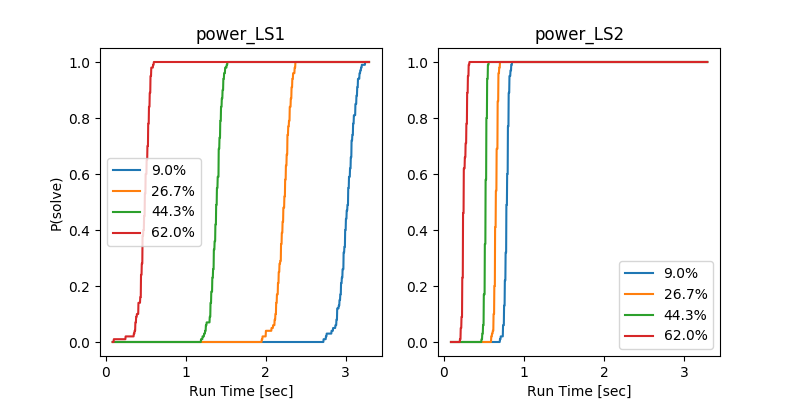
\includegraphics[width=400px]{plots/qrtd_power.png}
	\caption{QRTDs for \textit{power} Graph}
	\label{figure:qrtd_power}
\end{figure*}

\begin{figure*}[h]
	\centering
	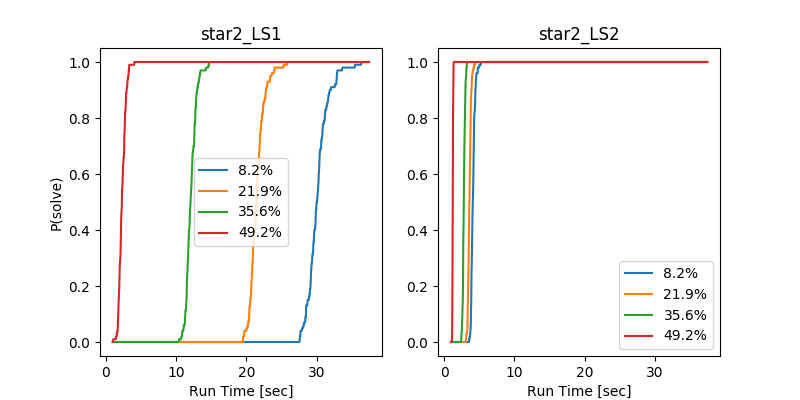
\includegraphics[width=400px]{plots/qrtd_star2.png}
	\caption{QRTDs for \textit{star2} Graph}
	\label{figure:qrtd_star2}
\end{figure*}

\begin{figure*}[h]
	\centering
	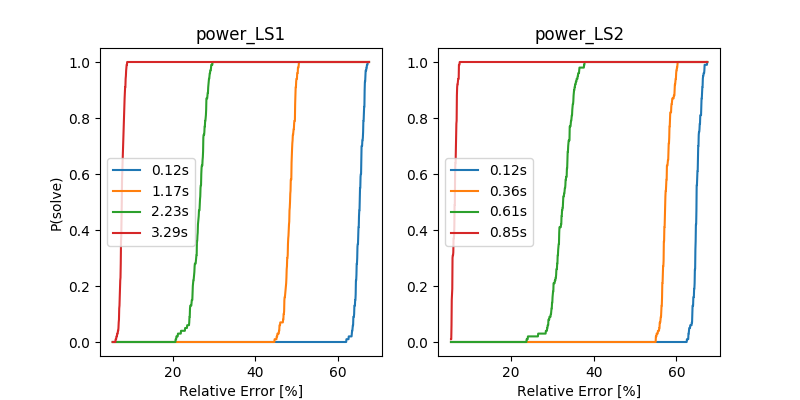
\includegraphics[width=400px]{plots/sqd_power.png}
	\caption{SQDs for \textit{power} Graph}
	\label{figure:sqd_power}
\end{figure*}

\begin{figure*}[h]
	\centering
	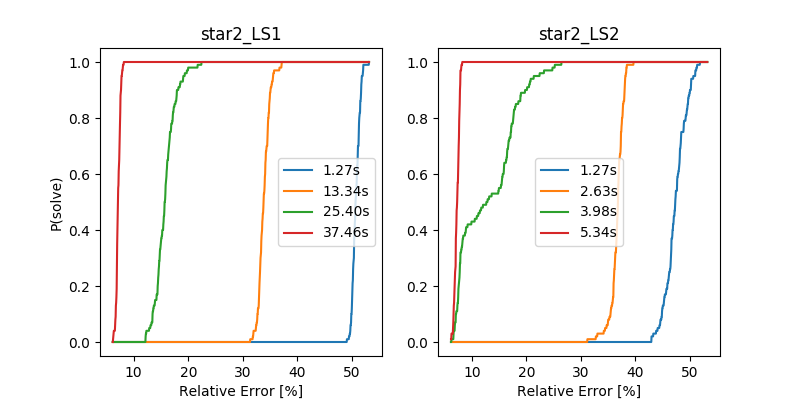
\includegraphics[width=400px]{plots/sqd_star2.png}
	\caption{SQDs for \textit{star2} Graph}
	\label{figure:sqd_star2}
\end{figure*}

\begin{figure}[h]
	\centering
	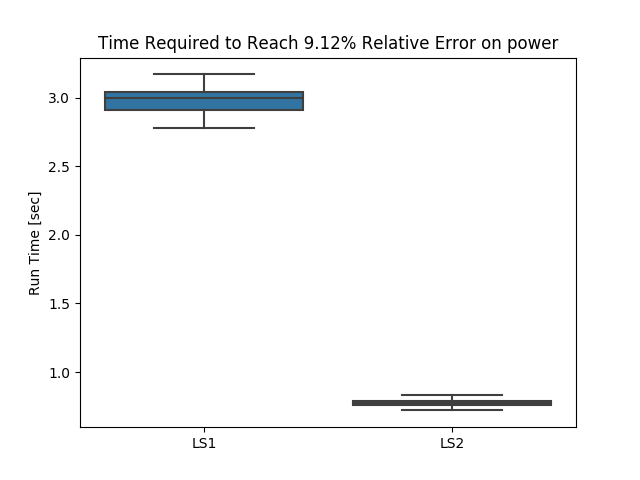
\includegraphics[width=250px]{plots/boxplot_power.png}
	\caption{Running Times for \textit{power} Graph}
	\label{figure:boxplot_power}
\end{figure}

\begin{figure}[h]
	\centering
	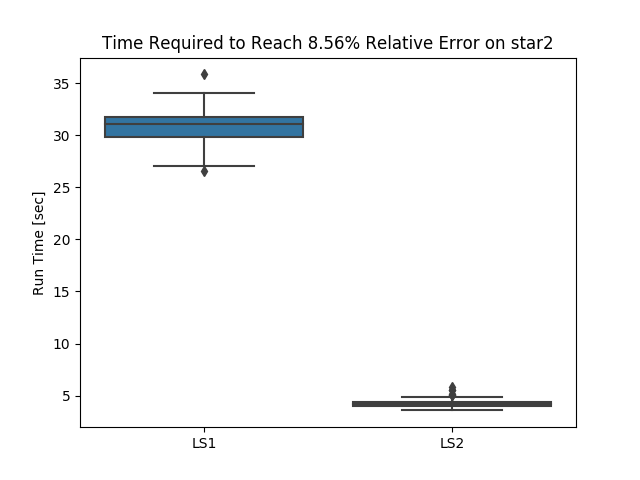
\includegraphics[width=250px]{plots/boxplot_star2.png}
	\caption{Running Times for \textit{star2} Graph}
	\label{figure:boxplot_star2}
\end{figure}

\section{Discussion}
As shown in Table \ref{table:algperf}, LOCAL-SEARCH-VC-2 obtains similar performance to LOCAL-SEARCH-VC-1 in significantly less time. On average, it takes about 53\% of the time to obtain a solution that has 1.06 times as much relative error. In two instances (email and power) LOCAL-SEARCH-VC-2 actually has lower relative error.

\section{Conclusion}

\bibliographystyle{ACM-Reference-Format}
\bibliography{citations} 

\end{document}